

\begin{figure}[t]\label{fig:curve_1_so3_example}
    \begin{subfigure}[t]{0.5\textwidth}
        \centering
        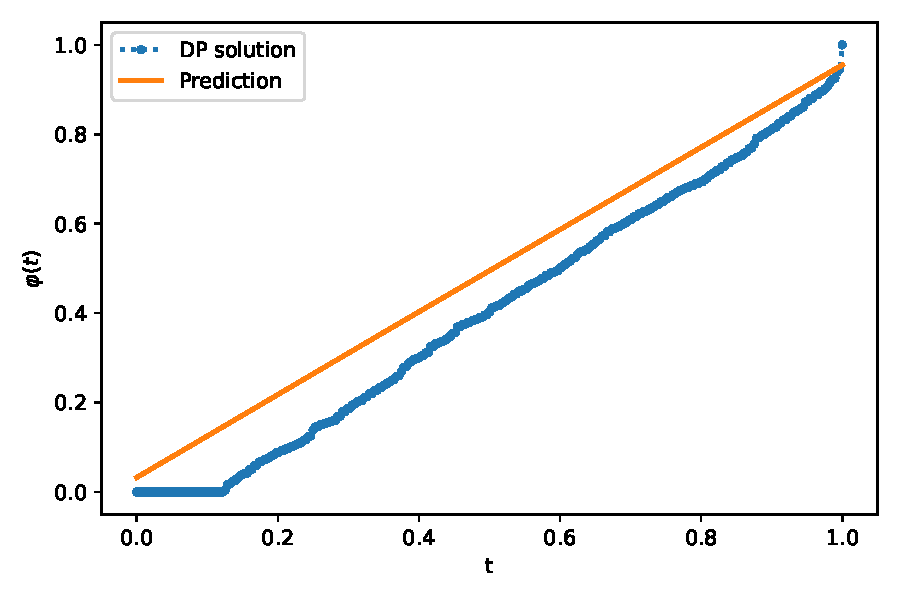
\includegraphics[width=\linewidth]{figures/curve_so3/pc_eks_2/plot_1_0.pdf}
        \caption{Solutions found by neural network training and dynamic programming.}
        \label{fig:curve_so3_pc_solution}
    \end{subfigure}a
    \begin{subfigure}[t]{0.5\textwidth}
        \centering
        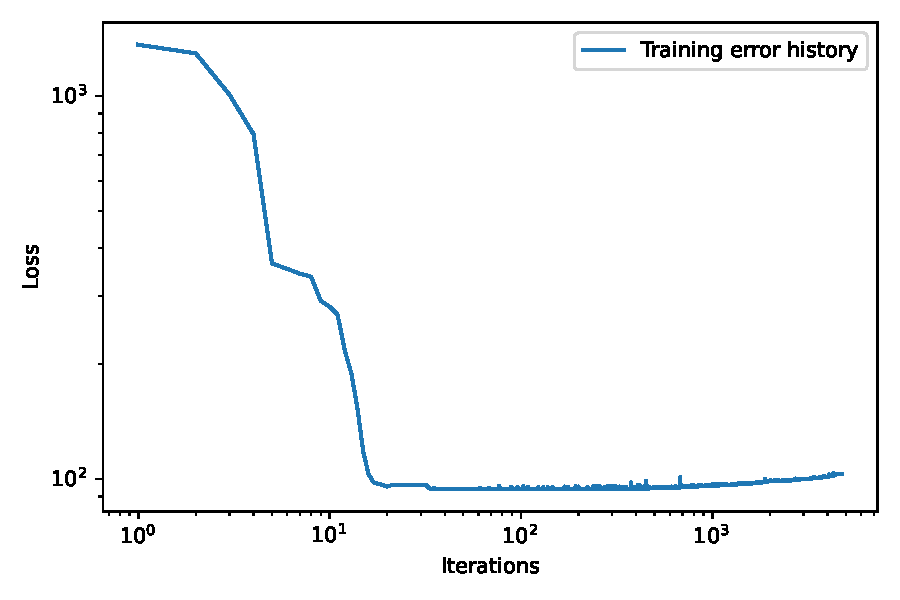
\includegraphics[width=\linewidth]{figures/curve_so3/pc_eks_2/history_plot_1.pdf}
        \caption{The cost function \(L(\theta)\) with each iteration.}
        \label{fig:curve_so3_pc_history}
    \end{subfigure}
    \begin{subfigure}[t]{0.5\textwidth}
        \centering
        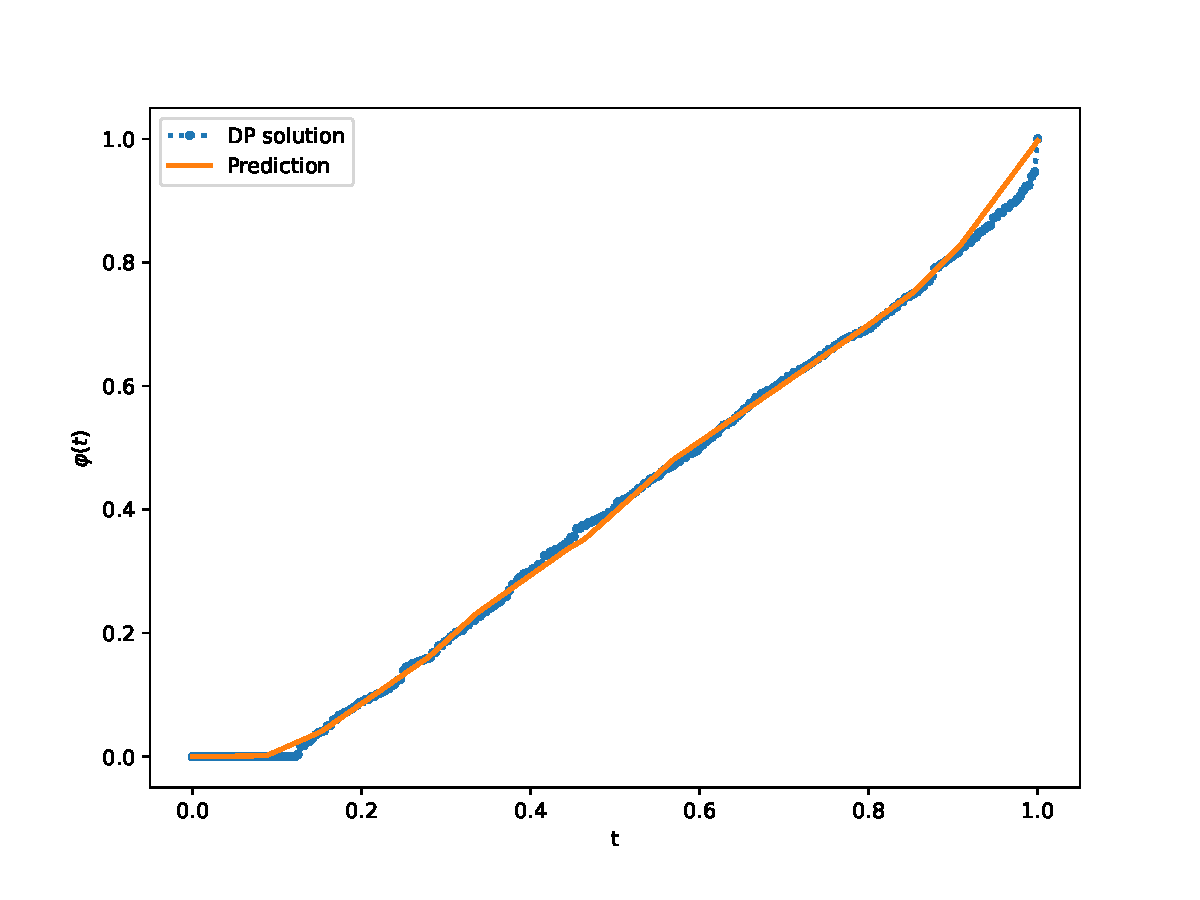
\includegraphics[width=\linewidth]{figures/curve_so3/pl_eks_6/plot_288_0.pdf}
        \caption{Solutions found by neural network training and dynamic programming.}
        \label{fig:curve_so3_pl_solution}
    \end{subfigure}
    \begin{subfigure}[t]{0.5\textwidth}
        \centering
        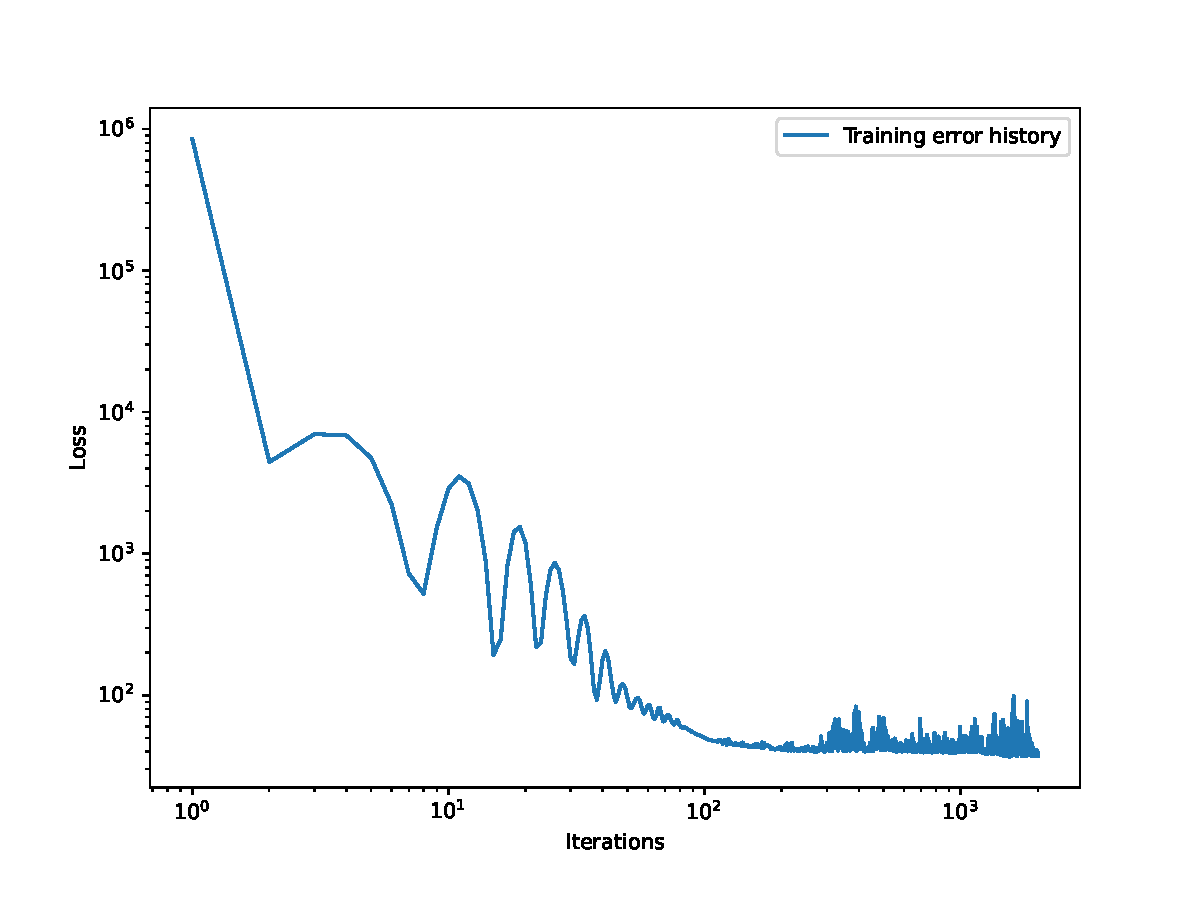
\includegraphics[width=\linewidth]{figures/curve_so3/pl_eks_6/history_plot_288.pdf}
        \caption{The cost function \(L(\theta)\) with each iteration.}
        \label{fig:curve_so3_pl_history}
    \end{subfigure}
    \caption{The approximate optimal reparametrizations of two curves representing motion capture data. Figure \ref{fig:curve_so3_pc_solution} shows the solution for the piecewise constant interpolation of the data, and Figure \ref{fig:curve_so3_pl_solution} shows the solution for the linearly interpolated curve. The approximate solutions are compared to the solution found by the dynamic programming algorithm and the corresponding training history is shown in the figure to the right.}
\end{figure}

\begin{figure}[t]\label{fig:curve_so3_pl_eks}
    \begin{subfigure}[t]{0.5\textwidth}
        \centering
        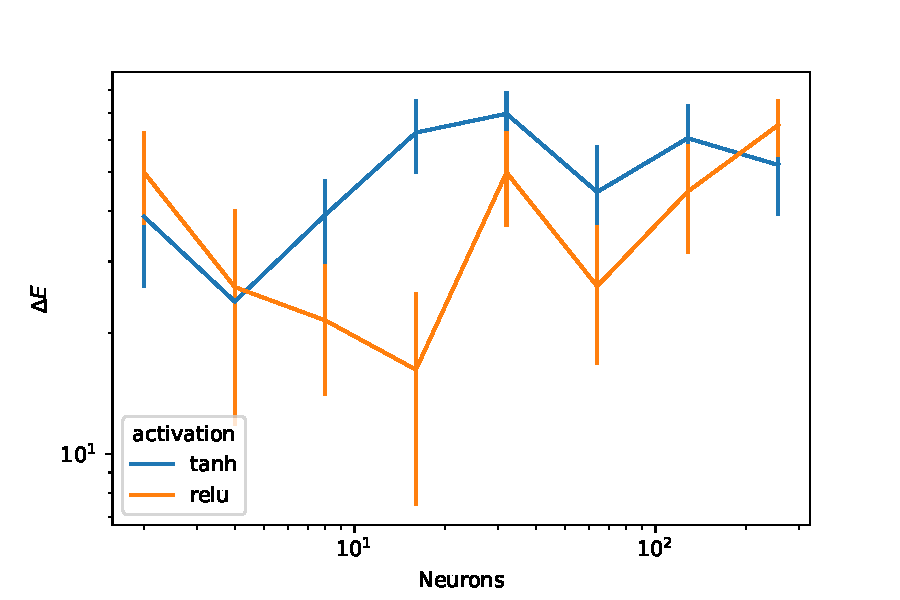
\includegraphics[width=\linewidth]{figures/curve_so3/pl_eks_6/neurons_error.pdf}
        \caption{The final cost \(E\) with the number of neurons in each hidden layer.}
        \label{fig:curve_so3_pl_neuron_error}
    \end{subfigure}
    \begin{subfigure}[t]{0.5\textwidth}
        \centering
        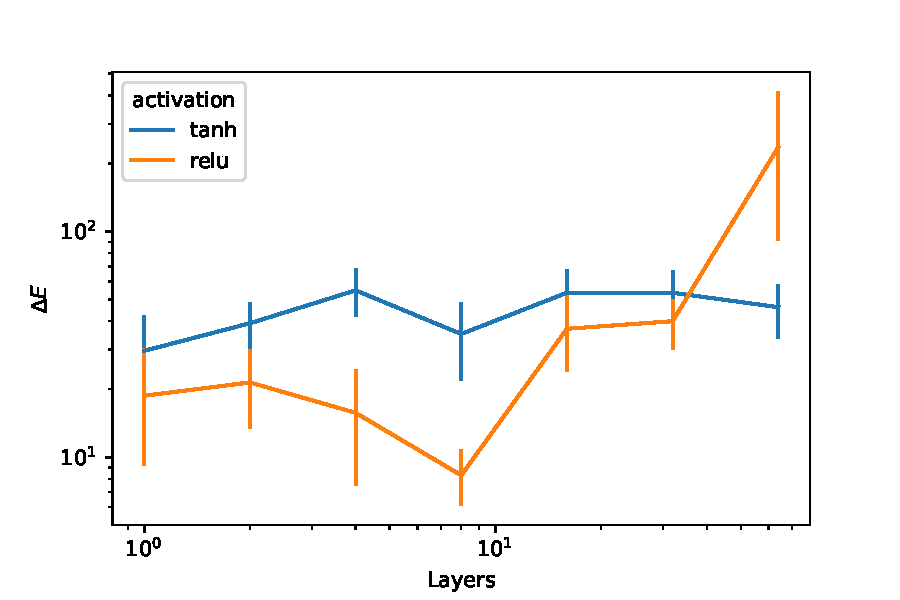
\includegraphics[width=\linewidth]{figures/curve_so3/pl_eks_6/layer_error.pdf}
        \caption{Final cost \(E\) with the number of layers.}
        \label{fig:curve_so3_pl_layer_error}
    \end{subfigure}
    \caption{Result of ensemble training for the piecewise linear version of the problem with curves generated by motion capture data with different number of neurons and hidden layers. In Figure \ref{fig:curve_2_neuron_error} the number of layers was fixed at 2. In Figure \ref{fig:curve_2_layer_error} the number of neurons is fixed at 8 per hidden layer. The error bars denote a 80\% confidence interval found by bootstrapping.}
\end{figure}

